\documentclass{WCCM-ECCOMAS_2026_Full_Paper}

\usepackage{graphicx}
\usepackage{amsmath}
\usepackage{booktabs}


\usepackage[colorlinks=true,linkcolor=blue,urlcolor=blue,citecolor=blue]{hyperref}

\title{Instructions to prepare a full paper for the 17th World Congress on Computational Mechanics \& 10th European Congress on Computational Methods in Applied Sciences and Engineering\\(WCCM-ECCOMAS 2026 Congress)}
\vspace{4pt}
\author{First A. Author$^{*}$, Second B. Author$^{\dagger}$ and Third C. Coauthor$^{\dagger}$}
\shortauthors{First A. Author, Second B. Author and Third C. Coauthor.}

\address{%
$^{*}$ International Center for Numerical Methods in Engineering (CIMNE)\\
Universitat Polit\`ecnica de Catalunya (UPC) Campus Nord,\\
08034 Barcelona, Spain\\
e-mail: congress@cimne.upc.edu, www.cimne.com\\[12pt]
$^{\dagger}$ German Association for Computational Mechanics (GACM)\\
Schinkelstra\ss e 2, 52062 Aachen, Germany\\
email: gacm@gacm.de, www.gacm.de}

\keywords{Computational Mechanics, FEM, Contact Problems.}

\summary{This document provides information and instructions for preparing a Full Paper to be included in the Proceedings of WCCM-ECCOMAS 2026 Congress}

\begin{document}

\maketitle

\section{Introduction}

All the participants whose Abstract has been accepted for presentation at the WCCM ECCOMAS 2026 Congress are kindly requested to submit the Full Paper (not mandatory) electronically via the web page of the \href{https://www.wccm-eccomas2026.org/}{Congress}, before \textbf{September 15\textsuperscript{th}, 2026}. Congress Proceedings (including full papers only) will be published on \href{https://www.scipedia.com/}{Scipedia} with DOI number after the congress and will be submitted for indexation to SCOPUS database. Submission of the full paper is not mandatory. The Full Paper should be written following the format of macros for submission. The file has to be translated into Portable Document Format (PDF) before submission via the Conference site. The organizers do not commit themselves to include in the Proceedings any Full Paper received later than the above-mentioned deadline. The corresponding author should be the speaker, and is expected to register and pay his registration fee during the advance period (before \textbf{September 15\textsuperscript{th}, 2026}) for the paper to be included in the technical programme of the WCCM-ECCOMAS 2026.

\section{General specifications}

The Full Paper must be written in English within a printing box of 16cm x 21cm, centered in the page. The Full Paper including figures, tables and references must have a minimum length of 6 pages and must not exceed 12 pages. Maximum file size is 4 MB.

\section{Title, authors, affiliation, key words}

The first page must contain the Title, Author(s), Affiliation(s), Key words and the Summary. The Introduction must begin immediately below, following the format of this template.

\subsection{Title}

The title should be written centered, in 14pt, boldface Roman, all capital letters. It should be single spaced if the title is more than one line long.

\subsection{Author}

The author's name should include first name, middle initial and surname. It should be written centered, in 12pt boldface Roman, 12pt below the title.

\subsection{Affiliation}

Author's affiliation should be written centered, in 11pt Roman, 12pt below the list of authors. A 12pt space should separate two different affiliations.

\subsection{Key words}

Please, write no more than six key words. They should be written left aligned, in 12pt Roman, and the line must begin with the words \textbf{Key words:} boldfaced. A 12pt space should separate the key words from the affiliations.

\subsection{Summary (optional)}

Use 12pt Italic Roman for the summary. The word \textbf{Summary} must be set in boldface, not italicized, at the beginning of the first line. The text should be justified and separated 12pt from the key words, as shown in the first page of these instructions.

\section{Headings}

\subsection{Main headings}

The main headings should be written left aligned, in 12pt, boldface and all capital Roman letters. There should be a 12pt space before and 6pt after the main headings.

\subsection{Secondary headings}

Secondary headings should be written left aligned, 12 pt, boldface Roman, with an initial capital for first word only. There should be a 12pt space before and 6pt after the secondary headings.

\section{Editorial heading}

The first page has to include the Editorial Heading, as shown in the first page of these instructions. Successive pages will include the name of the authors.

\section{Text}

The normal text should be written single-spaced, justified, using 12pt (Times New) Roman in one column. The first line of each paragraph must be indented 0.5cm. There is not inter-paragraph spacing.

\section{Page numbers}

In order to organize the Full Paper, it is better to number the pages. Page numbers are not included in the printing box.

\section{Figures}

All figures should be numbered consecutively and captioned. The caption title should be written centered, in 10pt Roman, with upper and lower case letters.

\begin{figure}[h!]
\centering
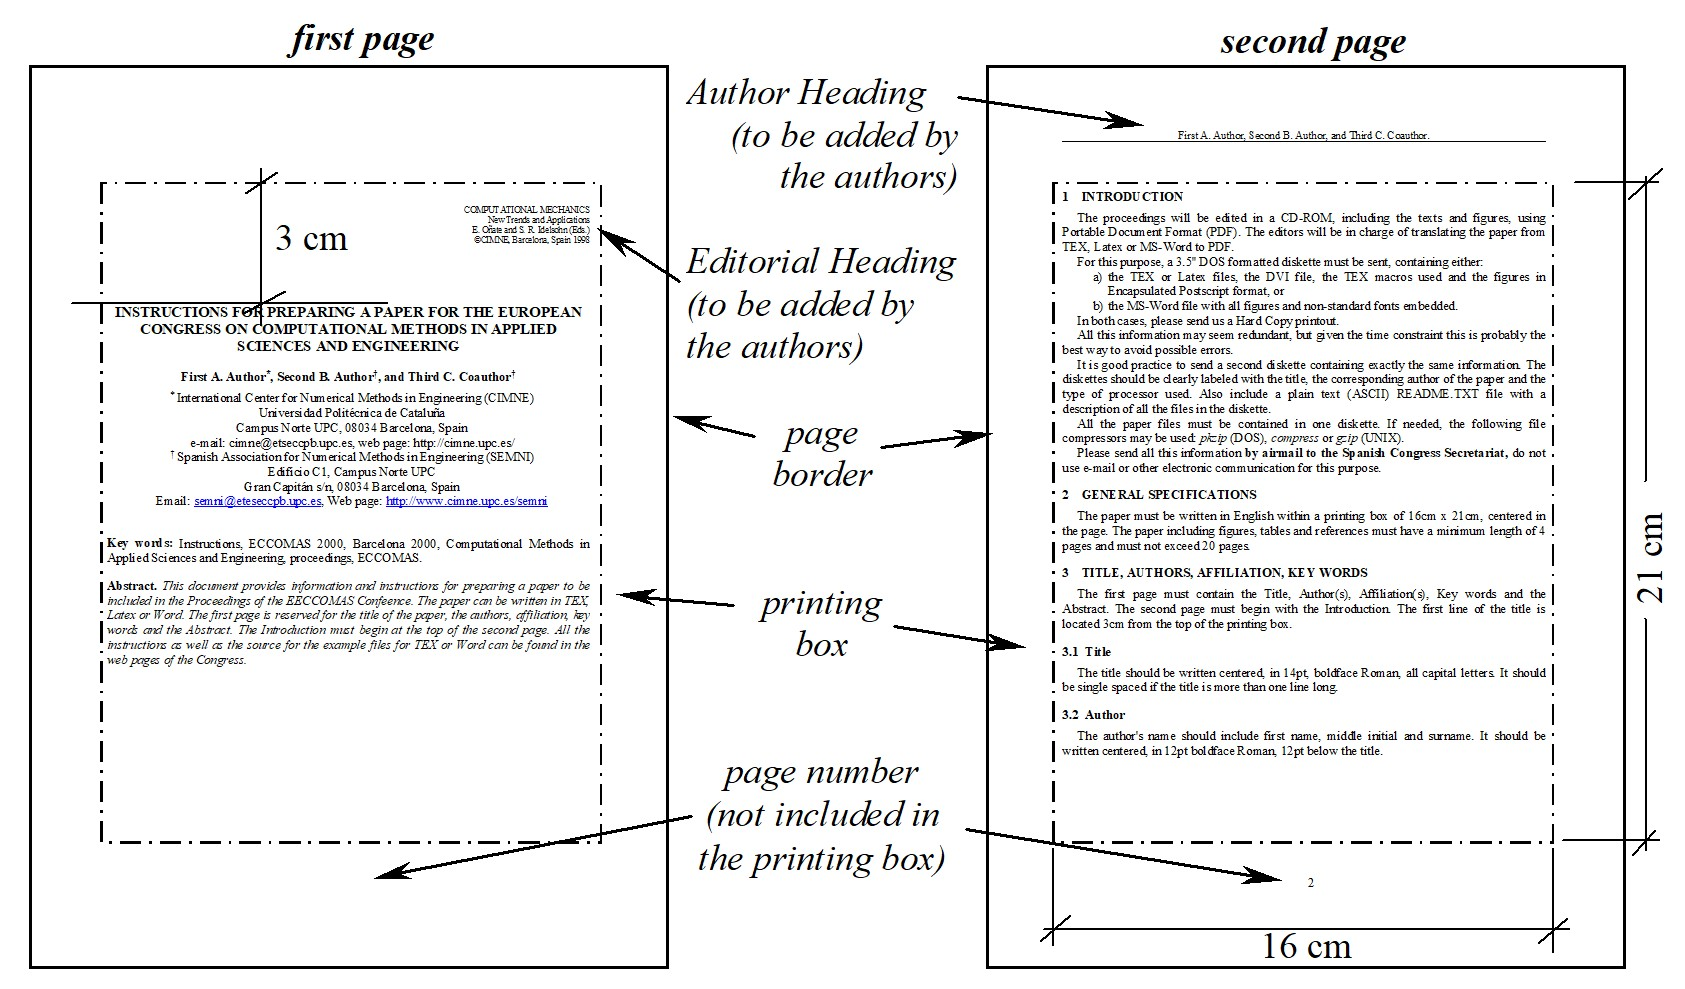
\includegraphics[width=1.0\textwidth]{figures/figure_example.jpg}
\caption{Page layout}
\label{fig:page-layout}
\end{figure}

A 6pt space should separate the figure from the caption, and a 12pt space should separate the upper part of the figure and the bottom of the caption from the surrounding text.
Figures may be included in the text or added at the bottom of the Full Paper.

\section{Equations}

A displayed equation is numbered, using Arabic numbers in parentheses. It should be centered, leaving a 6pt space above and below to separate it from the surrounding text.

The following example is a single line equation:

\begin{equation}
Ax=b
\end{equation}

The next example is a multi-line equation:

\begin{equation}
Ax=b
\end{equation}

\[
Ax=b
\]

\section{Tables}

All tables should be numbered consecutively and captioned, the caption should be 10pt Roman, upper and lower case letters.

\begin{table}[h!]
\centering
\caption{Example of the construction of one table}
\begin{tabular}{ccc}
\toprule
C11 & C12 & C13 \\
C21 & C22 & C23 \\
C31 & C32 & C33 \\
C41 & C42 & C43 \\
C51 & C52 & C53 \\
\bottomrule
\end{tabular}
\end{table}

A 6pt space should separate the table from the caption, and a 12pt space should separate the table from the surrounding text.

\section{Format of references}

References should be quoted in the text by superscript numbers [1,2] and grouped together at the end of the Full Paper in numerical order as shown in these instructions.

\section{Conclusions}

\begin{itemize}
\item Full Papers in format for publication should be submitted electronically via the web page of the Conference before \textbf{September 15\textsuperscript{th}, 2026}. They must be converted to Portable Document Format (PDF) before submission. The maximum size of the file is 4 Mb.
\end{itemize}

\begin{thebibliography}{2}

\bibitem{Zienkiewicz}
O.C. Zienkiewicz and R.L. Taylor, \textit{The finite element method}, McGraw Hill, Vol. I., (1989), Vol. II, (1991).

\bibitem{Laurin}
F. Laurin, N. Carr\`ere and J.F. Maire. A multiscale progressive failure approach for composite laminates based on thermodynamical viscoelastic and damage models. Composites Part A, Vol. 38, pp. 198-209, 2007.

\end{thebibliography}

\end{document}
